\section{\mc 従来手法のまとめ}
運動想起型BCIは、様々な特徴量抽出手法と分類手法を適宜組み合わせて構築されている。
数多くの手法が以下に示す脳波に関する知見を意識している。
\begin{itemize}
    \item 運動想起する身体部位に応じて、強く反応する頭皮領域は異なる。
    \item 事象関連脱同期は、特定の周波数領域に生ずる。
    \item 個人差や計測環境の影響を受けやすい。
\end{itemize}
空間フィルタや
バンドパスフィルタあるいは時間周波数解析を用いること、
また複数の分類手法を比較しなければならないことの理由が
上記の脳波の性質に集約されている。
このセクションでは、多数存在する運動想起型BCIの構築方法に関して、
統一的な視点に立って概観する。その後、従来手法全般に対する問題点を提示し、このチャプターを終える。

\subsection{\mc 特徴量の観点からの従来手法}
運動想起を1回行った際に計測された脳波を以下で表記する。
\begin{equation}
    X =(x_1, \cdots, x_N)\in \mathbb{R}^{M \times N}\    
\end{equation}
ここに\(M\)は電極の個数、\(N\)は計測時間点数である。
空間フィルタは\(W\in \mathbb R^{M \times M}\)によって
脳波を\(W^TX \in \mathbb R^{M \times N}\)と変換する。
通常は更に電極の軸に関して次元削減を行うが、ここでは単に線形変換とする(必要であれば、後に削除すれば良い)。
時間周波数解析\(h(\cdot)\)は時間的に局在する基底関数を\(K\)個準備した場合、
各時間\(n\)において信号を基底関数の重ね合わせで表現した際の係数\(h(X) \in \mathbb R^{M \times N \times K}\)へと変換する。
空間フィルタと時間周波数解析の両方を用いる場合には、以下の形式で表される特徴量を抽出する。
\begin{equation}
    Z = h(W^TX) \in \mathbb R^{M\times N \times K}
    \label{eq:EEGfeatures}
\end{equation} 
一方でフィルタバンクを用いるFBCSPなどは以下の形式で表すことができる。
\begin{eqnarray}
    && {\cal H}  =  \{ {\cal H}_1,\cdots, {\cal H}_K \} \\
    && \hat X_k  = {\cal H}_k(X) \in \mathbb R^{M\times N} \\
    && Z_k  = W_k^T{\cal H}_k(\hat X_k) \in \mathbb R^{M\times N} \\
    && Z  =  (Z_1,\cdots, Z_K) \in \mathbb R^{M\times N \times K}
    \label{eq:EEGfeaturesbandpass}
\end{eqnarray} 
ここに\({\cal H}\)はフィルタバンクであり、\(K\)はフィルタの個数に相当する。
いずれにしても、抽出される特徴量は\(Z\in \mathbb R^{M\times N \times K}\)という
3階テンソル(電極×時間×周波数)である。

A. S. Aghaei\cite{Ztfc}も同様のことに言及しており、脳波\(X\)から\(Z\in \mathbb R^{M\times N \times K}\)
を獲得する様々な手法について比較している。
更に\(Z\)が得られた後の次元削減および運動想起部位を出力する分類器も含め、
一連の手法に関して、
電極軸と周波数軸に対する双線形変換によるアプローチを提案している(図\ref{fig:fbcsp bilinear}(b,c))。
図中で``space"と表現されている単語は本論文中では電極に相当する。\(\Omega\)は運動想起部位であり、
\(\hat \Omega\)がBCIの予測出力である。
\begin{figure}
    \centering
    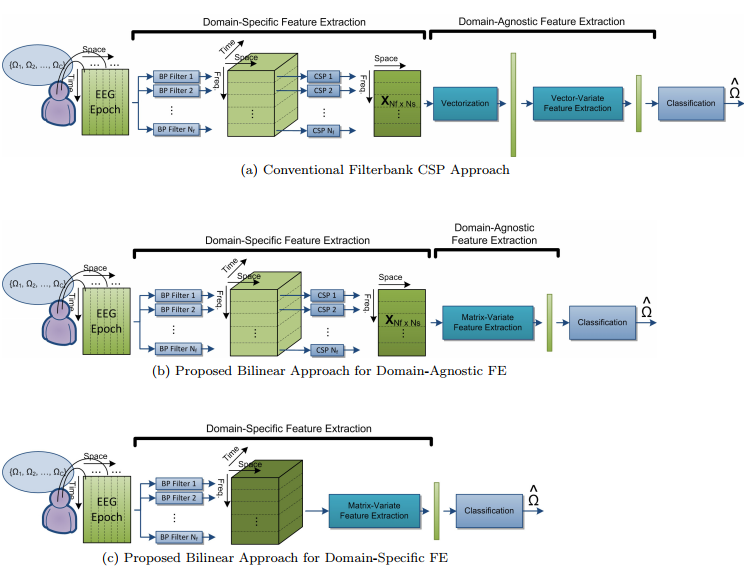
\includegraphics[width=14cm]{images/bilinear.png}
    \caption{脳波を3階テンソルとした手法の模式図(参照\cite{Ztfc})}
    \label{fig:fbcsp bilinear}
\end{figure}


\subsection{\mc 構成の観点からの従来手法}
次に典型的な運動想起型BCIの構成について述べる。
典型的な運動想起BCIは、運動想起に関連している脳波を取り出すための前処理\(\cal H(\cdot)\)
によって脳波の生データから\(\hat X\)を獲得することが一般的である。
\begin{equation}
    \hat X = {\cal H}(X)
    \label{eq:bandpass}
\end{equation}
次に、運動想起に関連している電極を選定するための空間フィルタ\(f(\cdot)\)を適用する。
\begin{equation}
    Z = f(\hat X)
    \label{eq:spatfilter}
\end{equation}
続いて\(Z\)に対して、
運動想起部位\(Y\)を出力する分類器\(g(\cdot)\)を準備することで、運動想起BCIが構成されている。
\begin{equation}
    Y = g(Z)
    \label{eq:classifier}
\end{equation}
従って、BCIは脳波\(X\)を引数とした合成関数という形式を取る。
\begin{equation}
    Y = (g\circ f \circ {\cal H})(X)
    \label{eq:bci_gosei}
\end{equation}
典型的なCSPを用いたBCIでは\(\cal H\)をバンドパスフィルタ、\(f\)をCSP、\(g\)をLDAやSVMによって個別に構成する。
ここで\(f^*(\cdot)=(f\circ{\cal H})(\cdot)\)として、バンドパスフィルタとCSPを同時に構成することを考えればCSSSPによるBCIになり、
\(\cal H\)をフィルタバンクにすることでFBCSPによるBCIとなる。
一方で時間周波数解析に基づくBCIでは変換(\ref{eq:time-freq})を\(h(\cdot)\)として、
\begin{equation}
    Y = (g\circ h \circ f \circ {\cal H})(X)
    \label{eq:bci_gosei2}
\end{equation}
という形式で表せる。この時、\(\cal H\)や\(f\)はERDを検出するための
神経科学的な知見に基づいた設計がなされる場合もあれば、機械学習の手法が用いられる場合もある。
更に時間周波数解析によって得られるパワースペクトログラムに対して
非負値行列分解などを用いて特徴量を抽出する試みもある\cite{kNMF,kNMF2}。
この場合も行列分解による変換を\(a(\cdot)\)と置けば
\begin{equation}
    Y = (g\circ a\circ h\circ f\circ {\cal H})(X)
    \label{eq:bci_gosei3}
\end{equation}
と表され、形式上は合成関数である。それぞれの関数の役割を明示しなければ、BCIは単に以下の合成関数である。
\begin{equation}
    Y = (f_K\circ \cdots \circ f_1)(X)
    \label{eq:bci_gosei4}
\end{equation}
BCIを合成関数(\ref{eq:bci_gosei4})を出発点にして見ると、
従来のBCI構築手法は、合成関数に含まれる関数の数を明確にし、
それぞれに役割を付与し、与えた役割を担うような調整が個々に行われていると見なせる。
ただし、関数\(f_i\)を設計するためには\(f_{i-1}\)の設計が終了していなければならない。

% 個々の関数\(f_i(\cdot)\)を設計する場合には、その候補となる関数族\(\{f_i(\cdot,\theta_i)\mid \theta_i \in \Theta_i\}\)を仮定する。
% ここに\(\Theta_i\)は\(\theta_i\)が取りうる全ての値の集合である。
% 例えば、CSPを用いた\(Y = (g_{lda}\circ f_{csp} \circ {{\cal H}_{buttord}})(X)\)で表されるBCIを考え、
% バタワースバンドパスフィルタ、CSP、LDAについて設計を行う場合は以下の関数族を仮定する。
% \begin{eqnarray}
%     {\cal H}_{buttord}(\cdot) &=& \{{\cal H}(\cdot,w_p,w_s,r_p,r_s) \mid w_p,w_s \in \mathbb R^2, r_p,r_s \in \mathbb R\} \\
%     \label{eq:H_buttord}
%     f_{csp}(\cdot) &=& \{f(\cdot, W_{csp})\ \mid W_{csp} \in \mathbb R^{m\times M} \}\\
%     \label{eq:f_csp}
%     g_{lda}(\cdot) &=& \{g(\cdot,W_{lda})\ \mid W_{lda} \in \mathbb R^{d \times m}\}    
%     \label{eq:g_lda}
% \end{eqnarray}
% \(w_p,w_s\)はそれぞれ通過帯域コーナー周波数、阻止帯域コーナー周波数である。
% \(r_p,r_s\)はそれぞれ通過帯域リップル、阻止帯域の減衰量である。
% \(W_{csp}\)はCSPにおける線形変換の表現行列であり、
% 電極数\(M\)の次元を持つ脳波を\(m (< M)\)の任意の次元の電極空間に圧縮する。
% \(W_{lda}\)はLDAにおける線形変換の表現行列であり、
% \(m\)次元の電極空間から分類クラスの数より小さな任意の\(d\)次元への射影を担う。
% ここではバンドパスフィルタのパラメータに関しては人手で決定され、
% CSPとLDAのパラメータはそれぞれの学習アルゴリズムによって決定される場合を想定する。
% ここで例に挙げたBCIは\({\cal H}_{buttord}\)の設計を終えなければ、\(f_{csp}\)の設計に入ることはできない。
% あるいは結果が期待通りでなかった場合には、\({\cal H}_{buttord}\)の設計に戻らなければならない。
% \({\cal H}_{buttord}\)が\(f_{csp}\)の学習結果にどのような影響を及ぼすのかは定かではないため、
% この後戻り設計は試行錯誤によって解決するしか無い。
% 一方でCSSSPはこの問題を解決した手法であると言えるが、
% 同様の問題が\(f_{lda}\)と\(f_{csp}\)の間にも存在する。



